\chapter{EXEMPLOS PARA UTILIZAÇÃO DO MODELO}
Este modelo foi desenvolvido para auxiliar no desenvolvimento do TCC dos estudantes dos cursos ofertados no IFSP - campus Birigui.

Aqui deve-se introduzir o trabalho. Trata-se da parte inicial do texto, onde devem constar: a delimitação do assunto tratado, os objetivos da pesquisa e outros elementos necessários para situar o tema do trabalho. 

No LaTeX, pule uma linha entre um parágrafo e outro para manter o espaçamento. Inserir $\setminus\setminus$ no final da linha, insere uma quebra de linha, mas não deixa parágrafo.\cite{adams1995}


\section{Criando uma seção} %Cria uma nova seção no texto
Para inserir uma nova seção no texto, utilize o comando $\backslash$section\{\}, inserindo o título da seção entre as chaves. Exemplo: para criar o título desta seção, utilize o comando:

$\backslash$section$\{$Criando uma seção$\}$\\

Para criar subseções, utilize os comandos a seguir:\\

$\backslash$subsection$\{$Criando uma subseção$\}$ \%cria uma subseção de nível 3

$\backslash$subsubsection$\{$Criando uma subseção$\}$ \%cria uma subseção de nível 4


\section{Citações e referências}
\onehalfspacing
Os comandos necessários para insrir uma citação no texto são explicados nesta seção. No arquivo .pdf você irá visualizar apenas o resultados final. Para saber qual comando utilizar para realizar a citação, verifique o arquivo cap0.tex.

Para inserir as referências utilizadas no texto, será utilizada a ferramenta BibTeX. Para isso, há um arquivo ref.bib no modelo. Nele, devem ser apresentadas as informações sobre as referências utilizadas´.

A formatação das referências foi definida no estilo do modelo e a utilização do BibTeX é por meio dos comandos que serão mostrados a seguir. Realizadas as citações, as referências serão apresentadas no final do texto, já no padrão definido pela ABNT 6023:2018 \cite{NBR6023}.

\subsection{Citação Direta}
Se o trecho da referência for utilizado de forma integral (Ctrl+C, Ctrl+V), deve ser realizada a citação direta, que pode ser curta (com menos de três linhas) ou longa (com três linhas ou mais)

\subsubsection{Citação direta curta}
Citação de até três linhas, entre aspas duplas com indicação da autoria, ano e página. No LaTeX, o texto citado deve ser inserido entre $\grave{}\grave{}$ e ". A citação utiliza o comando $\backslash$cite\{\}, sendo o marcador da referência indicado entre as chaves.

Exemplo:

A Lei n.$^o$ 10.695, de $1^o$ de julho de 2003 determina que a violação de direitos autorais é crime, com pena de ``detenção, de 3 (três) meses a 1 (um) ano, ou multa''  \cite{lei10695}.

\subsubsection{Citação direta longa}
Citação com mais de três linhas, com recuo de 4cm da margem esquerda, com letra menor que a do texto utilizado (fonte Arial, tamanho 10) e sem as aspas. Espaço simples (1,0 cm) entre as linhas, com indicação da autoria, ano e página.

No LaTeX, deve-se utilizar o ambiente quote\{\}, para identificar o texto a ser citado, o comando  $\backslash$small\{\}, para definir o tamanho da fonte, e o comando $\backslash$cite\{\} com o índice da referência, com a seguinte estrutura:\\
\begin{quote}
$\backslash$begin\{quote\}\\
$\backslash$small\{ SEU TEXTO AQUI \\
$\backslash$cite\{REFERÊNCIA\}\\
\}\\
$\backslash$end\{quote\}\\
\end{quote}

Exemplo:

O plágio é crime e a penalidade prevista para este tipo de crime é definida pela Lei n.$^o$ 10.695, de $1^o$ de julho de 2003:

\begin{quote}
\small{		
O art. 184 e seus §§ 1$^o$, 2$^o$ e 3$^o$ do Decreto-Lei n$^o$ 2.848, de 7 de dezembro de 1940, passam a vigorar com a seguinte redação, acrescentando-se um § 4$^o$:

        Art. 184. Violar direitos de autor e os que lhe são conexos:

        Pena – detenção, de 3 (três) meses a 1 (um) ano, ou multa.

        ...
        \cite{lei10695}}
\end{quote}

\subsection{Citação Indireta}
Citação baseada na ideia do autor consultado, ou seja, após ler o autor da obra, é extraída a ideia central dele, porém transcritacom as palavras do autor do trabalho. O autor da obra e ano devem ser citados.

A citação indireta no LaTeX é realizada com o comando $\backslash$cite\{\}, indicando a referência entre as chaves.

Exemplos:

A violação de direitos autorais é crime que pode resultar em detenção, de 3 (três) meses a 1 (um) ano, ou aplicação de multa \cite{lei10695}.

Em \cite{severo2018} foi realizado um estudo em relação ao comportamento do gás, como por exemplo de como é que se inicia a combustão, os seus impactos em relação ao ser humano físico, a inalação do gás toxico que é liberado na combustão.


\subsection{Citação da citação}
Citação direta ou indireta de um texto em que não se teve acesso ao original. Usa-se a expressão apud (citado por). No LaTeX, utilize o comando $\backslash$apudonline[ ]\{ \}\{ \}. Entre os colchetes deve constar o número da(s) página(s) em que aparece a citação na referência consultada. A referência original é inserida no primeiro par de chaves e a referência consultada, no segundo par de chaves.

Exemplo:

O Brasil é o terceiro país no ranking mundial de mortes por incêndio. Em 2015, foram contabilizadas 1349 ocorrências de incêndio, uma média de 112 por mês \apud[p.1]{sprinkler}{severo2018}.

\textbf{Nota:} A referência original, à qual não se teve acesso, deve ser definida no arquivo .bib como @hidden.


\section{Ilustrações e Tabelas}
Ilustrações e tabelas são inseridas no texto como elementos flutuantes, ou seja, que podem ser posicionados de forma distinta à do texto. Nesta seção serão apresentados alguns comandos que podem ser utilizados para inserir esses elementos no texto.

\subsection{Ilustrações}
Ilustrações podem ser desenhos, esquemas, quadros, fotografias, gráficos, mapas, imagens retiradas da internet, dentre outros. Segundo a NBR 14724 \cite{NBR14724}, a identificação das ilustrações aparece na parte superior, composta pela palavra designativa (figura, mapa, fluxograma, etc.) seguida de seu número de ordem de ocorrência no texto, em números arábicos, travessão e o respectivo título. Após a lustração, na parte inferior, deve-se indicar a fonte consultada (elemento obrigatório), legenda, notas e outras informações que sejam necessárias, alinhadas à esquerda da figura. 

No LaTeX, uma figura pode ser inserida utilizando-se o ambiente \textbf{figure}, com a seguinte estrutura:\\
\begin{quote}
$\backslash$begin\{figure\}[POSIÇÃO]\\
$\backslash$centering\\
$\backslash$textbf\{$\backslash$caption\{TÍTULO DA FIGURA\\
$\backslash$label\{RÓTULO DA FIGURA\}\}\}\\
	$\backslash$includegraphics[DIMENSIONAMENTO]\{NOME DO ARQUIVO\}$\backslash\backslash$\\
	$\backslash$legend\{$\backslash$footnotesize$\backslash$textbf\{Fonte:\} FONTE DA FIGURA\}\\
$\backslash$end\{figure\}\\
\end{quote}

Exemplo:

A frequência  dos estudantes nas disciplinas optativas é mostrada na Figura \ref{fig:freq}.

\begin{figure}[!ht]
\textbf{\caption{Frequência  dos estudantes nas disciplinas optativas\label{fig:freq}}}
	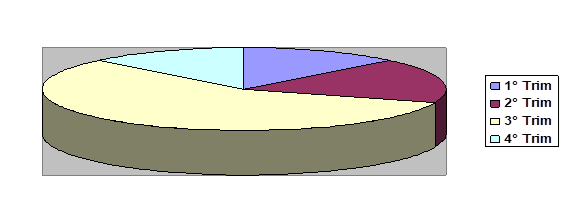
\includegraphics[scale=1.25]{imagens/grafico.png}
	\captionsetup{singlelinecheck=false}
	\legend{\hspace{1cm}\footnotesize\textbf{Fonte: }elaborado pelo autor.}
\end{figure}

As informações que devem ser inseridas nos comandos são apresentadas a seguir.

\subsubsection{Posicionamento da figura no texto}
\label{posiciona}
Nos colchetes ao lado do comando $\backslash$begin\{figure\}[ ] deve ser inserida a informação sobre a posição da figura, da seguinte maneira:

h - para inserir a figura exatamente neste ponto do texto

t - para inserir a figura no topo da página

b - para inserir a figura na base da página



\normalsize
p - para inserir a figura na página\\

Mais de uma opção pode ser utilizada, sendo que a ordem das letras representa a ordem de preferência de posicionamento. Colocar um sinal de exclamação (!) antes das letras significa que o compilador deve forçar o atendimento da configuração definida pelo usuário.

\subsubsection{Título e rótulo da figura}
O título da figura deve ser inserido entre as chaves do comando $\backslash$caption\{ \}. O LaTeX irá numerar a figura automaticamente e apresentar sua numeração e título.

O rótulo da figura é inserido com o comando $\backslash$label\{ \} e serve de identificação para que a figura seja encontrada pelo LaTeX. O rótulo não é mostrado no texto, mas utilizada todas as vezes que queremos chamar a figura ou falar sobre ela. 

\subsubsection{Incluindo a figura}
O comando $\backslash$includegraphics[ ]\{ \} insere a figura no ambiente. Entre os colchetes deve ser informado o dimensionamento da figura. Algumas possibilidades são:

\textbf{width=num} - define a largura da figura. A variável num, após o sinal de igualdade, indica o valor da largura definida para a figura. Deve ser informada a unidade, que pode ser mm, cm, in, pt...

\textbf{height=num} - define a altura da figura.

\textbf{scale=num} - redimensiona a figura na escala definida com base em suas dimensões originais. É possível diminuir (num < 1) ou amentar a figura (num > 1).

\textbf{angle}=num - rotaciona a figura em sentido anti-horário. O argumento \textbf{num} deve informar o ângulo de rotação em graus.

\textbf{width=scale$\backslash$textwidth} - define a largura da figura com relação à largura do texto

\textbf{width=scale$\backslash$paperwidth} - define a largura da figura com relação à largura do papel

\textbf{height=scale$\backslash$paperheight} - define a altura da figura com relação à altura do papel

Entre as chaves deve ser informado o nome do arquivo. Caso a figura esteja em uma subpasta ou em uma pasta diferente dos arquivos .tex, deve-se informar o caminho até a pasta onde está o arquivo  da figura.

\subsubsection{Legenda da figura}
Na legenda, deve-se informar a fonte de onde a figura foi retirada. Caso seja de autoria própria, deve-se escrever ``Elaborado pelo autor''. Caso tenha sido retirada de alguma referência, deve-se fazer a citação dessa referência, utilizando-se o comando $\backslash$cite\{ \}.


\subsubsection{Chamada da figura no texto}
As ilustrações devem ser chamadas no texto, utilizando-se o comando $\backslash$ref\{ \}, inserindo-se o rótulo (label) da figura entre as chaves.

\subsection{Tabelas}
A inserção de tabelas no texto utiliza os ambientes \textit{table} e \textit{tabular}. No primeiro, são definidos elementos como o título, o rótulo e a posição da tabela no texto. Os comandos $\backslash$caption\{ \} e $\backslash$label\{ \}, utilizados com figuras, aplicam-se também a tabelas. As instruções para posicionamento mostradas em \ref{posiciona} também servem para tabelas. No ambiente \textit{tabular} são inseridos os valores que preenchem a tabela, utilizando o símbolo \& como separador de colunas e $\backslash\backslash$ como separador de linhas.

Como as tabelas podem possuir diferentes especificações de linhas e colunas, seguem alguns exemplos:\\

As inclinações recomendadas para os módulos fotovoltaicos para diferentes latitudes são mostradas na Tabela \ref{tab:inclina}.

\begin{table}[h]
\textbf{\caption{Inclinações recomendadas para os módulos fotovoltaicos\label{tab:inclina}}}
\centering
\begin{tabular}{c|c}
\toprule
Latitude geográfica do local & Ângulo de inclinação recomendado \\
\hline
$0^o$ a $10^o$  & $\alpha = 10^o$\\
$0^o$ a $10^o$  & $\alpha = latitude$\\
$0^o$ a $10^o$  & $\alpha = latitude + 5^o$\\
$0^o$ a $10^o$  & $\alpha = latitude + 10^o$\\
acima de $40^o$ & $\alpha = latitude + 15^o$\\
\bottomrule
\end{tabular}
\legend{\footnotesize\textbf{Fonte: }\cite{garcia2020}}
\end{table}

Na Tabela \ref{tab:partes} está esquematizado o padrão recomendado pela NBR 14724 \cite{NBR14724}, que foi elaborado para facilitar a apresentação formal dos trabalhos acadêmicos, na ordem exata em que os elementos devem ser apresentados:

\begin{table}[h]
\bfseries{\caption{Partes que compõem a estrutura do TCC}\label{tab:partes}}
\normalfont
\begin{tabular}{|l|l|l|}
\hline
\multicolumn{2}{|l|}{Parte externa}                                                                     & \begin{tabular}[c]{@{}l@{}}\textbf{Capa}\\\underline{Lombada}\vspace{0.5cm}\end{tabular}                                                                                                                                                                                                                                                                                                                                                                         \\ \hline
\multirow{3}{*}{Parte interna} & \begin{tabular}[c]{@{}l@{}}Elementos\\pré-textuais\end{tabular} & \begin{tabular}[c]{@{}l@{}}\textbf{Folha de rosto}\\\textbf{Ficha catalográfica (no verso da folha de rosto)}\\\underline{Errata}\\\textbf{Folha de aprovação}\\\underline{Dedicatória}\\  \underline{Agradecimentos}\\\underline{Epígrafe}\\\textbf{Resumo na língua vernácula}\\\textbf{Resumo em língua estrangeira}\\\underline{Lista de ilustrações}\\\underline{Lista de tabelas}\\\underline{Lista de abreviaturas e siglas}\\\underline{Lista de símbolos}\\\textbf{Sumário}\end{tabular} \\ \cline{2-3} 
                               & \begin{tabular}[c]{@{}l@{}}Elementos\\textuais\end{tabular}     & \begin{tabular}[c]{@{}l@{}}\textbf{Introdução}\\\textbf{Desenvolvimento}\\\textbf{Conclusão}\end{tabular}                                                                                                                                                                                                                                                                                                                                         \\ \cline{2-3} 
                               & \begin{tabular}[c]{@{}l@{}}Elementos\\pós-textuais\end{tabular} & \begin{tabular}[c]{@{}l@{}}\textbf{Referências}\\\underline{Glossário}\\\underline{Apêndice(s)}\\\underline{Anexo(s)}\\\underline{Índice}\end{tabular}                                                                                                                                                                                                                                                                                                            \\ \hline
\multicolumn{3}{|l|}{\begin{tabular}[c]{@{}l@{}}\textbf{Elementos obrigatórios}\\\underline{Elementos opcionais}\end{tabular}}                                                                                                                                                                                                                                                                                                                                                                                                                               \\ \hline
\end{tabular}
\legend{\footnotesize\textbf{Fonte:} adaptada de \cite{NBR14724}} %Indicar a autoria da Tabela
\end{table}

\textbf{Nota: }para inserir tabelas no texto é possível utilizar os assistentes do TexMaker. A explicação de como utilizá-los está na série de vídeo-aulas.


\section{Expressões Matemáticas}
Expressões matemáticas, como fórmulas, sistemas de equações, matrizes, etc., podem ser inseridas na mesma linha do texto ou à parte dele, dando maior destaque à expressão. Nesta seção serão mostradas algumas formas de se construir essas expressões no texto.

\subsection{Fórmulas na mesma linha do texto}
Para inserir uma fórmula simples na mesma linha do texto, basta escrever a expressão entre \$\$. Exemplo:

Para um triângulo retângulo, pode-se escrever que $a^2+b^2=c^2$, sendo $a$ e $b$ os catetos e $c$ a hipotenusa do triângulo.


\subsection{Fórmulas destacadas do texto}
As expressões matemáticas podem ser destacadas do texto para facilitar a leitura. Se necessário pode-se numerá-las com algarismos arábicos entre parênteses alinhados à direita, como (\ref{eq1}) e (\ref{eq2}). Para as fórmulas é permitida uma entrelinha maior para comportar os expoentes e índices. Para destacar as expressões do texto, utiliza-se o ambiente \textbf{equation}. Para chamar as expressões no texto, é necessário nelas colocar um rótulo, utilizando o comando $\backslash$label\{ \} logo após iniciar o ambiente equation.

Exemplos:\\

\noindent
$\backslash$begin\{equation\}\\
$\backslash$label\{eq1\}\\
x\string^2+x\string^3=n\\
$\backslash$end\{equation\}\\

retorna:

\begin{equation}
\label{eq1}
x^2+x^3=n
\end{equation}

Já o código:\\

\noindent
$\backslash$begin\{equation\}\\
$\backslash$label\{eq2\}\\
x=$\backslash$frac\{-b $\backslash$pm $\backslash$sqrt\{$\backslash$Delta\}\}\{2.a\}\\
$\backslash$end\{equation\}

retorna:

\begin{equation}
\label{eq2}
x=\frac{-b \pm \sqrt{\Delta}}{2.a}
\end{equation}

Os caracteres especiais, como símbolos matemáticos e letras gregas são inseridos por comandos, como $\backslash$pm, que insere o sinal de mais/menos ou $\backslash$Delta, que insere a letra grega $\Delta$. Contudo, é possível utilizar os assistentes do Texmaker para inserir esses símbolos sem que seja necessário memorizar todos os comandos.

Caso a expressão não precise ser numerada, utilize o ambiente \textbf{$\backslash$equation*}. Exemplo:\\

\noindent
$\backslash$begin\{equation*\}\\
$\backslash$label\{eq3\}\\
V\_\{Lmed\} = 0,225 $\backslash$times (1-cos$\backslash$beta)\\
$\backslash$end\{equation*\}\\

retorna:

\begin{equation*}
\label{eq3}
V_{Lmed} = 0,225 \times (1-cos\beta)
\end{equation*}

\subsection{Expressões longas}
Caso a expressão a ser apresentada seja muito longa, é possível quebrá-la e inseri-la em mais de uma linha utilizando o ambiente \textbf{multiline}. A quebra da equação não é automática e deve ser definida pelo usuário.\\

\noindent
$\backslash$begin\{multline\}\\
p(x) = 3x\string^6 + 14x\string^5y + 590x\string^4y\string^2 + 19x\string^3y\string^3 - 10x\string^3y\string^2 + 6x\string^2y\string^5 + 33x\string^2y\string^4$\backslash\backslash$\\ 
- 12x\string^2y\string^3 - 12xy\string^5 + 2y\string^6 - a\string^3b\string^3\\
$\backslash$end\{multline\}\\

retorna:\\
\begin{multline}
p(x) = 3x^6 + 14x^5y + 590x^4y^2 + 19x^3y^3 - 10x^3y^2 + 6x^2y^5 + 33x^2y^4\\ 
- 12x^2y^3 - 12xy^5 + 2y^6 - a^3b^3\\
\end{multline}

\subsection{Conjuntos de expressões}
Quando for necessário alinhar várias equações, pode-se utilizar o ambiente \textbf{align}. O símbolo $\&$ indica o ponto de alinhamento entre as equações. Assim, o código:\\

\noindent
$\backslash$begin\{align\}\\
3x + 2y + 5z $\&$ = 10$\backslash\backslash$\\
2x - y + 3z $\&$ = 4$\backslash\backslash$\\
2y + z $\&$ = 6
$\backslash$end\{align\} \\

Retorna as expressões alinhadas no sinal de igualdade:

\begin{align}
3x + 2y + 5z &= 10\\
2x - y + 3z &= 4\\
2y + z &= 6 
\end{align}

Outra opção é a utilização do ambiente \textbf{$\backslash$array}, que pode ser utilizado para alinhar expressões ou para construir matrizes ou outras estruturas em que exista a necessidade de alinhamento. A principal vantagem seste ambiente em comparação com o ambiente $\backslash$align é que ele permite o alinhamento de vários pontos na expressão, utilizando o símbolo \&. Além disso, ele permite determinar se o alinhamento será à esquerda (\textbf{l}eft), centralizado (\textbf{c}enter) ou à direita (\textbf{r}ight). Porém, ele deve ser inserido em um ambiente matemático, por exemplo, o ambiente equation. Exemplos:

O mesmo sistema de equações anterior pode ter todos os seus termos alinhados utilizando o código a seguir.\\

\noindent
$\backslash$begin\{equation\}\\
$\backslash$begin\{array\}\{rrrlr\}\\
3x \&+ 2y \&+ 5z \&= \&10$\backslash\backslash$\\
2x \&- y \&+ 3z \&= \&4$\backslash\backslash$\\
\&2y \&+ z \&= \&6 \\
$\backslash$end\{array\}\\
$\backslash$end\{equation\}

Tem-se, então a saída a seguir. Observe que os termos das equações estão alinhados à direita, mantendo o alinhamento nas variáveis.

\begin{equation}
\begin{array}{rrrlr}
3x &+ 2y &+ 5z &= &10\\
2x &- y &+ 3z &= &4\\
&2y &+ z &= &6 
\end{array}
\end{equation}

O valor de uma função para diferentes condições pode ser mostrado, por exemplo:\\

\noindent
$\backslash$begin\{equation\}\\
|x| = $\backslash$left$\backslash$\{ $\backslash$begin\{array\}\{ll\}\\
         x \& $\backslash$mbox\{if \$x $\backslash$geq 0\$\};$\backslash\backslash$\\
        -x \& $\backslash$mbox\{if \$x < 0\$\}.\\
        $\backslash$end\{array\} $\backslash$right.\\
$\backslash$end\{equation\}\\

retorna: 

\begin{equation}
|x| = \left\{ \begin{array}{ll}
         x & \mbox{if $x \geq 0$};\\
        -x & \mbox{if $x < 0$}.
        \end{array} \right. 
\end{equation}

Agora, um exemplo de montagem de uma matriz. O código a seguir retorna a matriz \ref{matriz}.\\

\noindent
$\backslash$begin\{equation\}\\
$\backslash$left[ $\backslash$begin\{array\}\{ccc\}\\
a \& b \& c $\backslash\backslash$\\
d \& e \& f $\backslash\backslash$\\
g \& h \& i $\backslash$end\{array\} $\backslash$right]\\
$\backslash$end\{equation\}

\begin{equation}
\label{matriz}
\left[ \begin{array}{ccc}
a & b & c \\
d & e & f \\
g & h & i \end{array} \right]
\end{equation}

